\documentclass{article}
\author{Junseo Shin, Sean Wang}
\date{}
\title{Computational Fluid Dynamics}

\usepackage{custom}
\usepackage{lipsum}
\graphicspath{{../../data/}}
%\usepackage{subcaption} % for subfigures
% set figure numbering to Fig. 1, Fig. 2, etc.
\renewcommand{\thefigure}{\arabic{figure}}

\begin{document}

\maketitle
% \tableofcontents
% \pagebreak

%CHAPTER 1
% \subfile{chapters/chapter1}

\section*{Introduction}
In this project, we implemented a 2D fluid solver using the finite volume method to solve the Euler equations (reduced from the governing Navier-Stokes equation) for the time evolution of fluids.
We solve the Euler equations in a 2D box $L_x \times L_y = 1 \times 1$ discretized into $N_x \times N_y = 514 \times 514$ cells with ghost cells at the boundary (therefore 512 $\times$ 512 physical cells)
faciliated by periodic boundary conditions, so that the flow of the fluid will wrap around at the boundaries. The \texttt{.h} header files contain the computational method for solving the fluid equations,
and output the data to a \texttt{.csv} file at each time step. The \texttt{.cpp} files contain the main function to run the simulation for a simple sound wave or the Kelvin-Helmholtz instability which
can help us understand phenomena visible in atmospheres of Jupyter near the Giant Red Spot.

\section*{Sound Waves in a Fluid}
For a simple test case to verify that our fluid solver works as intended and to test the stability of the simulation,
we simulated a 2D soundwave in a fluid with a sinusoidal density perturbation.
For sound soundwave we chose to simulate an ideal monoatomic gas---i.e. an adiabatic index $\gamma = 5.0 / 3.0$---initial density $\rho_0 = 1$, initial pressure $P_0 = 1$,
and sinusoidal density perturbation $\rho_1 = \num{e-3} \sin(6\pi x)$. 
From the equation of states, we can define the speed at which the density fluctuations travel by
\begin{align*}
    c = \sqrt{\gamma P_0 / \rho_0} = \sqrt{5.0 / 3.0} \approx 1.29.
\end{align*}
To estimate this velocity using the simulation data, we can track the position of one of the wave crests and measure
the time it takes to travel back to its initial position.
After this time $t$, the wave will have traveled a across 512 physical units, or the full length of the domain $L_x = 1.0$,
so we can use the simple velocity formula $v = \Delta x / \Delta t$ to estimate the velocity of the wave.
From the simulation data, the wave travels back to its initial position at $t \approx 0.77$, so the estimated velocity is
\begin{align*}
    c_{\text{est}} = \frac{1.0}{0.77} \approx 1.30
\end{align*}
This estimate has a perecent error of $\frac{1.30 - 1.29}{1.29} \times 100\% \approx 1\%$ compared to the theoretical value,
so our simulation agrees with the theory even for a low resolution of 512x512 physical unit cells.

% figure ../../data/sound_wave/cmax_output_rho_77.png
\begin{figure}[htbp]
    \centering
    \begin{subfigure}{0.31\textwidth}
        \centering
        \includegraphics[width=\textwidth]{sound_wave/cmax_output_rho_c4_t200.png}
        \caption{$C_{\text{CFL}} = 0.4$ (unstable)}
    \end{subfigure}
    \hfill
    \begin{subfigure}{0.31\textwidth}
        \centering
        \includegraphics[width=\textwidth]{sound_wave/cmax_output_rho_77_stable.png}
        \caption{$C_{\text{CFL}} = 0.5$ (stable)}
    \end{subfigure}
    \hfill
    \begin{subfigure}{0.31\textwidth}
        \centering
        \includegraphics[width=\textwidth]{sound_wave/cmax_output_rho_77_unstable.png}
        \caption{$C_{\text{CFL}} = 0.6$ (unstable)}
    \end{subfigure}
    \caption{512x512 resolution density plot of the soundwave at time $t$ for different CFL factors.}
    \label{fig:soundwave}
\end{figure}

\subsection*{CFL Condition}
The Courant-Friedrichs-Lewy (CFL) condition has a dimensionless factor $C_{\text{CFL}}$ that determines the stability of a given
numerical scheme. While running the soundwave simulation for different time intervals and CFL factors, we found that
even for small values of $C_{\text{CFL}}$, the simulation would become unstable if the time interval was too large. For example,
at $C_\text{CFL} = 0.4$, the simulation became visibly unstable at around $t = 2.0$ (Fig. \ref{fig:soundwave}a).
Furthermore, \texttt{sound\_wave\_c2.mp4} shows the simulation at $C_{\text{CFL}} = 0.2$ ran for longer time, and the shape of the soundwave
breaks down by $t = 7.0$.

So with this in mind, we confined the time interval to $t=0.77$ which is the approximate time interval it takes for a wave crest to
travel and return to its initial position.
After testing several values of the CFL factor $C_{\text{CFL}}$,
we found that the simulation was stable until we reached a maximum value of $C_\text{max} \approx 0.5$.
Moreover, when we set $C_{\text{CFL}} = 0.5$, the simulation was stable, but when we increased it to $C_{\text{CFL}} = 0.6$,
the output at $t=0.77$ becomes unstable,and the waves look like they break up into smaller waves and the structure of the initial soundwave becomes 
unrecognizable (Fig. \ref{fig:soundwave}c) by the end of the simulation.


% NOTES: 
% exec file description:
% - swtest1: C_cfl = 0.4, t = 5.0
% - swtest2: C_cfl = 0.6, t = 1.0
% - swtest3: C_cfl = 0.5, t = 1.0
% - swtest4: C_cfl = 0.2, t = 5.0

% KH stuff
% - 512x512
% - KH TIME: 145s
% - KHMP TIME: 80s
% kh_growth_first.png: C=0.4, rho_d=4, rho_0=1, v0=0.5, k=6
% kh_growth_k1.png: C=0.4, rho_d=4, rho_0=1, v0=0.5, k=1
% kh_growth_k4.png: C=0.4, rho_d=4, rho_0=1, v0=0.5, k=4
% kh_growth_k8.png: C=0.4, rho_d=4, rho_0=1, v0=0.5, k=8
% kh_growth_k12.png: C=0.4, rho_d=4, rho_0=1, v0=0.5, k=12
% kh_slow.mp4: C=0.2, rho_d=4, rho_0=1, v0=0.5, k=6
% kh_low_c.mp4: C=0.2, rho_d=4, rho_0=1, v0=0.5, k=2


\section*{Kelvin-Helmholtz Instability}


Kelvin-Helmholtz (KH) instability develops when 2 fluids of different
densities meet each other. To simulate the fluid trajectories, we
initialized a screen with x, y dimensions set to 1.0 x 1.0 using 512x512
resolution (defined by $N_x$ and $N_y$ which each include 2 ghost cells) similar 
to the soundwave simulation.
Each position within the matrix corresponds to the mass density at that
point. We used the following variables:
\begin{align*}
    a = 0.25;b = 0.75;\; \rho_{d} = 4;\; \rho_{0} = 1;\; v_{0} = 0.5;\;
    P_{0} = 2.5;\; k = 6.0\pi;\; v_\text{small} = 0.01;\; \sigma = 0.05
\end{align*}
Importantly, $a$ and $b$ describe the respective lower and upper boundaries
where the 2 different fluids meet. To generate the initial condition for
the KH wave, we used the following initial conditions:
\begin{align*}
    a \leq y \leq b:\quad         \rho &= \rho_d,\quad v_x= v_0 \\
    y < a \textrm{ or } y > b:\quad \rho &= \rho_0,\quad v_x = -v_0
\end{align*}
These initial conditions generate a slab of density \(\rho_d\)
surrounded by regions of density \(\rho_0\) with the fluids moving in
opposite conditions. We then introduced a sine-wave velocity profile in
the y direction to trigger instability at the boundary between both
fluids:
\begin{align*} \tag{1} \label{eq:vy}
    v_y = v_\text{small} \sin(kx) \qt(
        e^{-(y - a)^2 / \sigma^2} + e^{-(y - b)^2 / \sigma^2}
    )
\end{align*}
To parallelize the finite volume method, we added the \texttt{\#pragma omp
parallel for collapse(2)} directive at the start of each for-loop in the
finite volume solver. However, we were surprised to only see a
$\sim$2x improvement in speed, whereas our speed improved
significantly when we parallelized the code for the black hole project.
This was probably bottlenecked by the csv \texttt{output()} function
which writes the density data to a new file at each output time step \texttt{output\_dt = 0.01}.


% \includegraphics[width=6.5in,height=2.12917in]{media/image1.emf}

% \textbf{Figure 3:} KH waves at different time stamps where increasing
% color brightness represents increasing density.
% figure ./images/kh3.png
\begin{figure}[htbp]
    \centering
    \includegraphics[width=0.8\textwidth]{images/kh3.png}
    \captionsetup{width=0.8\textwidth}
    \caption{KH waves at different time stamps where increasing
    color brightness represents increasing density.}
    \label{fig:kh3}
\end{figure}

At the start the simulation, we see a high-density slab surrounded by
low density regions \textbf{(Figure 2A)}. By time $t = 1.00$, an ordered
pattern of vortices with $\lambda \sim 0.35$ \textbf{(Figure 2B)}.
This is very close (maybe even exact) to the predicted wavelength of 1/3
which is calculated from $\lambda = 2\pi / k$ where $k$ is the wavenumber that we
specified. As time progresses, the vortices become larger and wider, but
the wavelength remains the same \textbf{(Figure 2C)}. It should be noted
that the high density and low-density regions seem to mix.

As we can see in Figure \ref{fig:kh3}, the number wavelengths, or the number of swirling vortices, is
is equal to the wavenumber divided by $2\pi$, $k / 2\pi = 3$. Furthermore,
in the \texttt{kh\_k12.mp4} video where we change the wavenumber to $k = 12\pi$,
we can clearly see 6 swirling patterns form at the interfaces. When we
take $k = 100 \pi$ (\texttt{kh\_k100.mp4}), the swirling patterns disappear and the movie is 
quite boring to watch. However, this happens because the wavelength $\lambda = 2\pi / k = 0.02$
is too short to be captured by the simulation resolution of 512x512 physical cells, so
we would have to increase the resolution to capture the instability at this wavelength.

\subsection*{Random noise}

To check the effect of the initial $v_y$ perturbation, we
changed the sine-wave instability condition to a random number generator \texttt{rand}
that assigns a random wave number between 0 and $12\pi$ to each
$v_y$, so \eqref{eq:vy} becomes
\begin{align*}
    v_y = v_{\text{small}} \sin(\text{\texttt{rand}} \times x) \qt(
        e^{-(y - a)^2 / \sigma^2} + e^{-(y - b)^2 / \sigma^2}
    )
\end{align*} 
This leads to the formation of a disordered pattern of vortices with
undefined wavelengths \textbf{(Figure 3A, 3B)}. This makes sense since
we are introducing a perturbation at many different wavelengths rather
than a fixed one.

% \includegraphics[width=5.82778in,height=2.77442in]{media/image2.png}

% \textbf{Figure 4:} KH waves using k=6π, \(\rho_{d}\)=4, \(\rho_{0}\)=1
% and a initial randomized wavenumber.
% figure ./images/kh2.png
\begin{figure}[htbp]
    \centering
    \includegraphics[width=\textwidth]{images/kh2.png}
    \captionsetup{width=0.8\textwidth}
    \caption{KH waves using $k = 6\pi$, \(\rho_{d} = 4\), \(\rho_{0} = 1\)
    and a initial randomized wavenumber}
    \label{fig:kh2}
\end{figure}

% figure ./images/kh_growth_k1.png ... kh_growth_k12.png
\begin{figure}[htbp]
    \centering
    \begin{subfigure}{0.31\textwidth}
        \centering
        \includegraphics[width=\textwidth]{images/kh_growth_k1.png}
        \caption{}
    \end{subfigure}
    \hfill
    \begin{subfigure}{0.31\textwidth}
        \centering
        \includegraphics[width=\textwidth]{images/kh_growth_k4.png}
        \caption{}
    \end{subfigure}
    \hfill
    \begin{subfigure}{0.31\textwidth}
        \centering
        \includegraphics[width=\textwidth]{images/kh_growth_k6.png}
        \caption{}
    \end{subfigure}
    \begin{subfigure}{0.31\textwidth}
        \centering
        \includegraphics[width=\textwidth]{images/kh_growth_k8.png}
        \caption{}
    \end{subfigure}
    \begin{subfigure}{0.31\textwidth}
        \centering
        \includegraphics[width=\textwidth]{images/kh_growth_k12.png}
        \caption{}
    \end{subfigure}
    \captionsetup{width=0.8\textwidth}
    \caption{Growth of Kelvin-Helmholtz instability for different $k$ at 512x512 resolution.
    $\rho_0 = 1$, $\rho_d = 4$ (therefore $\delta = 3$), and theoretical growth curve $v_y = 0.002 e^{\sigma t}$ for all simulations.}
    \label{fig:kh_growth}
\end{figure}

\newpage
\subsection*{Growth rate and wave number}

The theoretical growth rate of the Kelvin-Helmholtz instability for the initial $v_y$ perturbation at the interfaces $a$ and $b$ is proportional to an exponential function
\begin{align*}
    v_y \propto e^{\sigma t}, \quad \sigma = \frac{2\sqrt{1 + \delta}}{2 + \delta} k v_0
\end{align*}
where $\rho_d = (1 + \delta) \rho_0$ is the higher density side. In order to align the growth rate curve to the simulation results,
we started with the $k = 6\pi$ cases and added a constant of of proportionality $D = 0.002$ to the theoretical growth rate $v_y = D e^{\sigma t}$.
This constant $D$ was mostly determined by trial and error, but we found that $D = 0.002$ was a good fit for the $k = 4\pi$ and $k = 8\pi$ cases as well,
so we used this value for all the theoretical growth rate curves.

Figure \ref{fig:kh_growth} shows that at $k =  6\pi, 8\pi$, the growth rate follows the theoretical prediction closely 
until around $t = 1.0$ where the $\abs{v_y}$ begins to plateau and the instability becomes nonlinear.
This nonlinear growth is expected as the vortices eventually merge and the fluid becomes more mixed and turbulent.
For $k = \pi$, the growth rate does not follow the theoretical prediction which may be due to the long wavelength $\lambda = 2\pi / k = 2$
not being able to capture the sinusoidal perturbation at the interfaces $a$ and $b$ very well.
For $k = 12\pi$, the max $\abs{v_y}$ quickly falls away from the theoretical growth after $t \sim 0.2$, and 
here, the wavelengths may be getting too short for the simulation resolution to capture the the growth
of the instability for an extended period of time.

\newpage
\subsection*{Density contrasts}

Next, we checked the influence of the 2 different fluid densities on the
KH wave. Swapping \(\rho_{d}\) and \(\rho_{0}\) only inverts the
direction of the vortices and the density of each fluid region
\textbf{(Figure 5A, 5B, 5D, 5E)}. When we set \(\rho_{d}\) =
\(\rho_{0}\), the vortices appear much quicker and is recognizable by t
= 0.31 \textbf{(Figure 5G)}. As time evolves, we see homogenous mixing
of both fluids and the vortices are spherical shaped rather than
elongated \textbf{(Figure 5C, 5F)}. Interestingly, changing the
\(\rho_d:\rho_0\) ratio does not or barely affect the shape of the
simulated growth rate curve \textbf{(Figure 5H)}. However, for our
\(\rho_{d}\) = \(\rho_{0}\) and swapped conditions, the theoretical
growth rate deviates more than the original condition from $t = 0.10$ to
1.00 \textbf{(Figure 5H).} These results demonstrate that fluid density
does not significantly affect the KH instability growth rate.

% \includegraphics[width=6.25in,height=6.04167in]{media/image3.emf}

% \textbf{Figure 5:} KH waves with different density regions

% figure ./images/kh1.png
\begin{figure}[htbp]
    \centering
    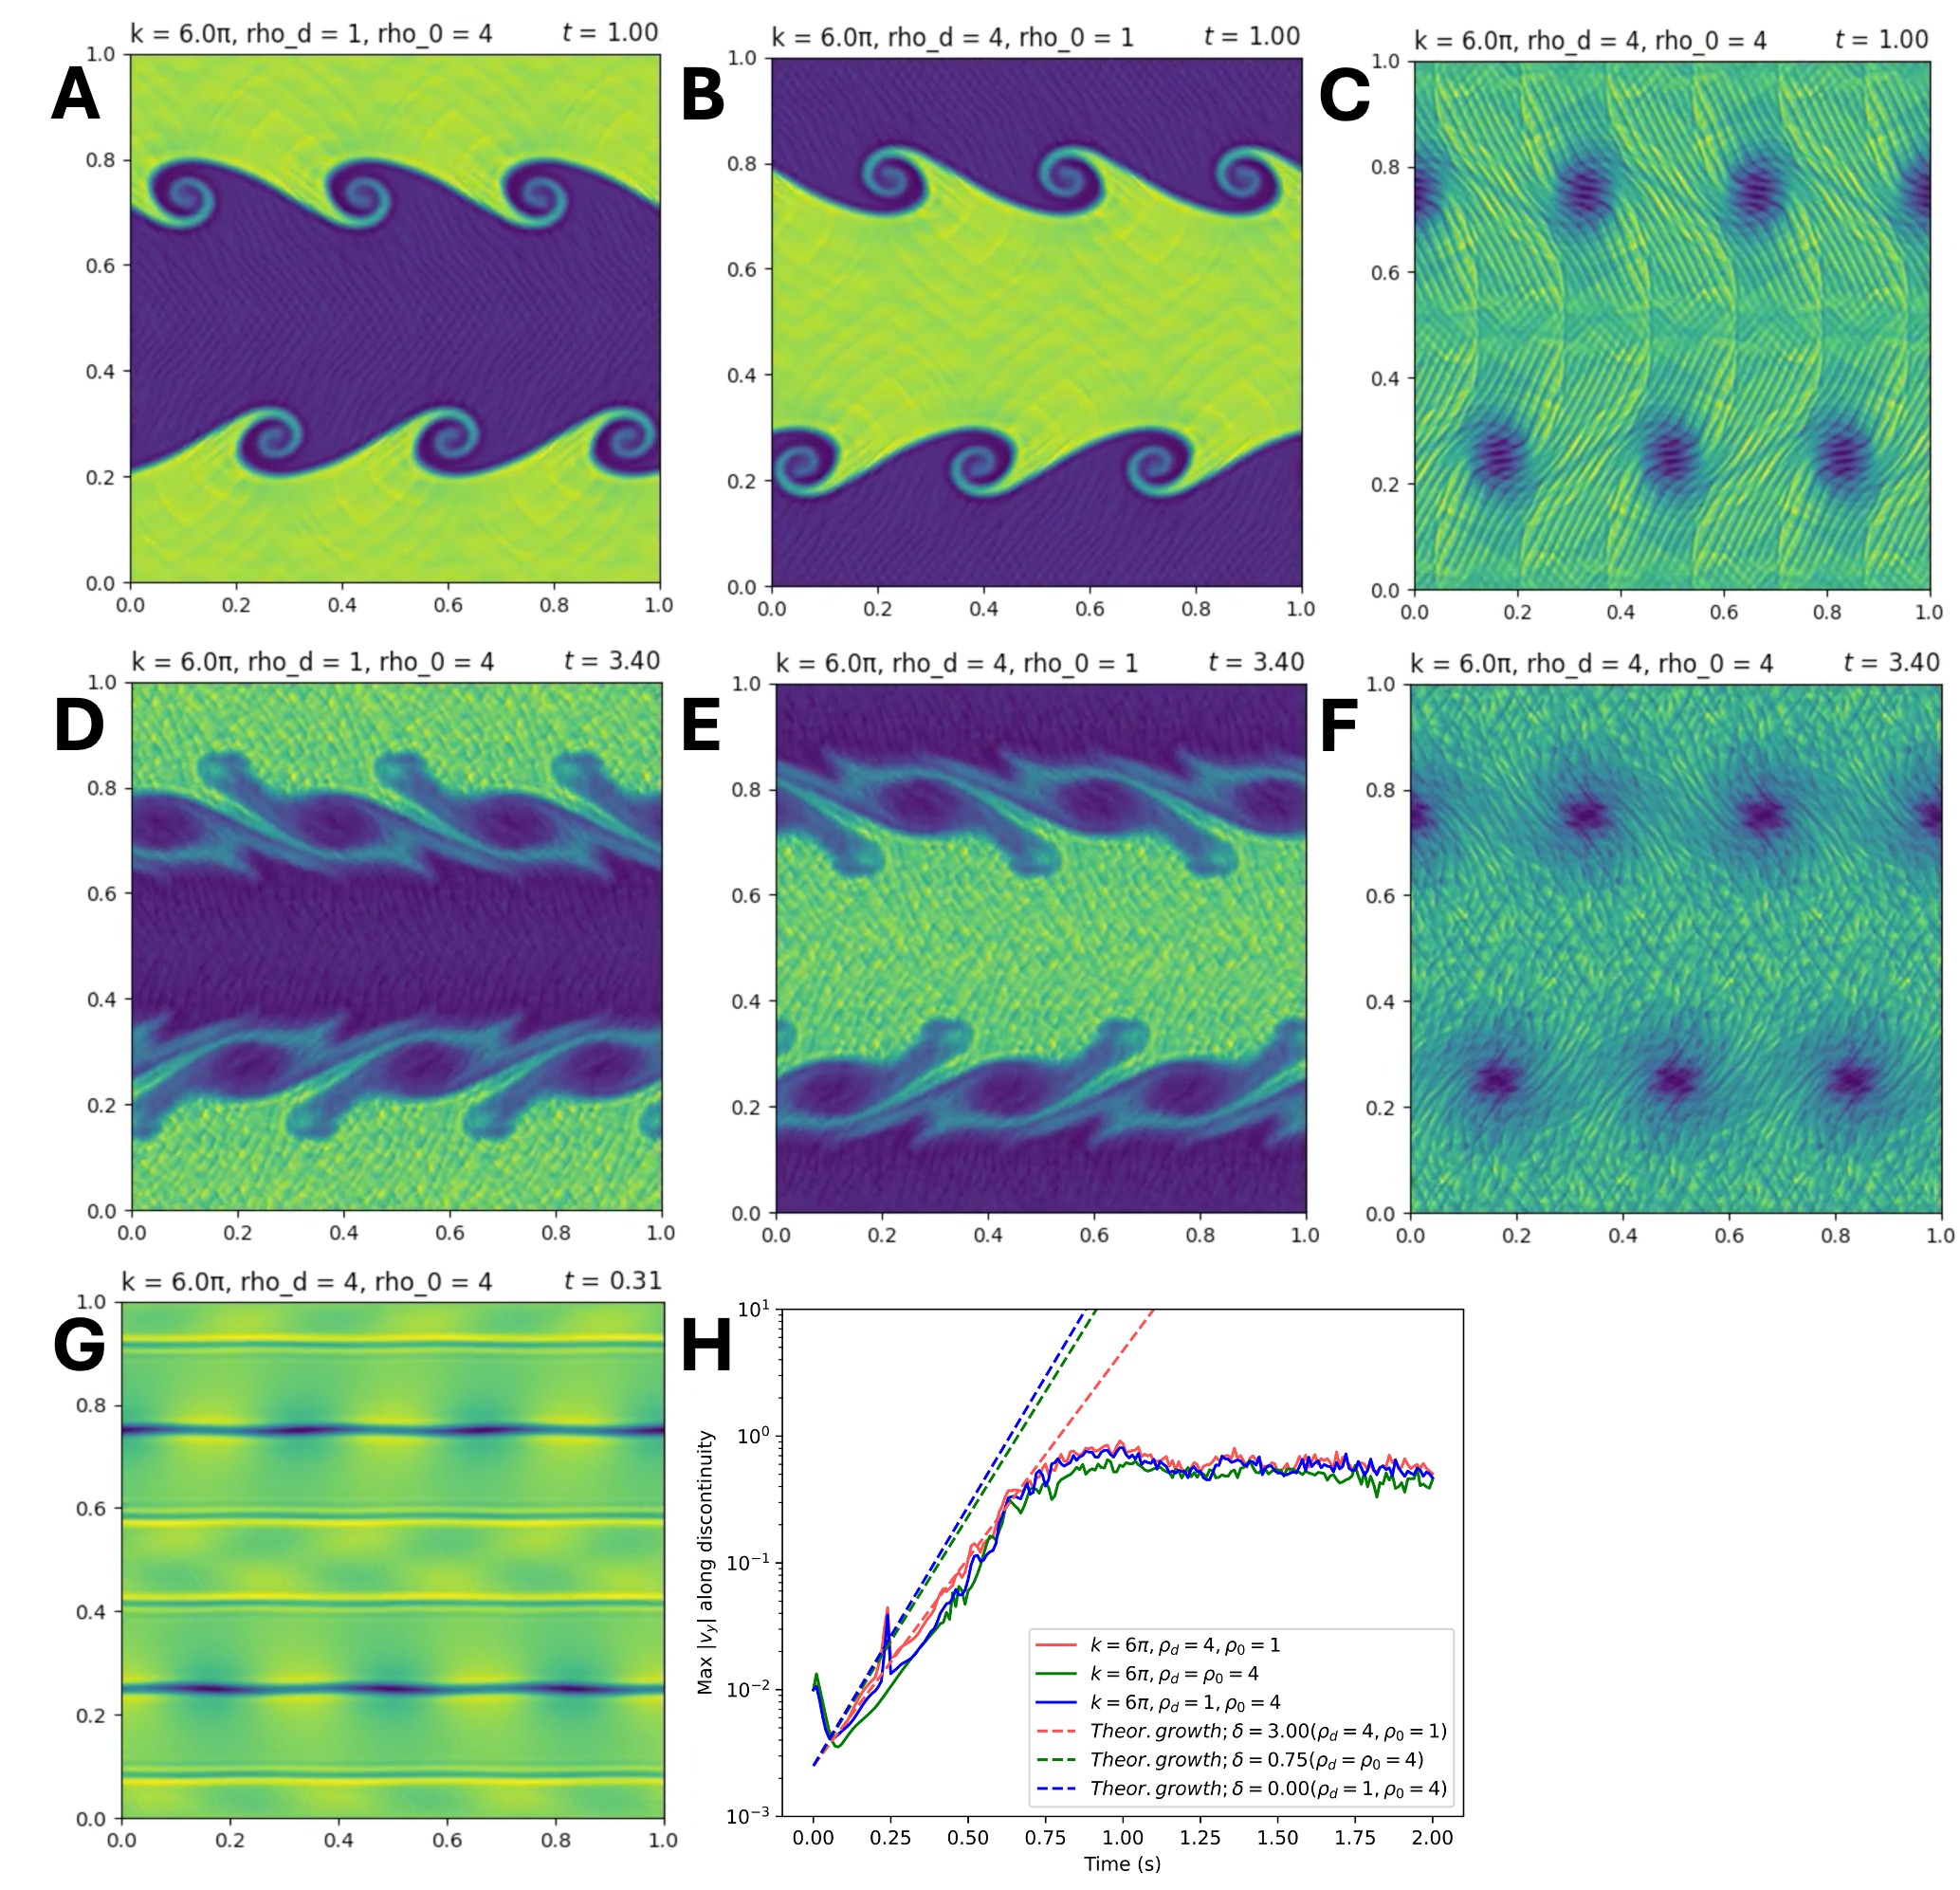
\includegraphics[width=\textwidth]{images/kh1.png}
    \caption{KH waves with different density regions}
    \label{fig:kh1}
\end{figure}
\end{document}




















% figure /einsteins_rings/EINSTEIN_RINGS.png
% \begin{figure}[ht]
%     \centering
%     \includegraphics[width=\textwidth]{/einstein_rings/EINSTEIN_RINGS.png}
%     \caption{Photon trajectory in Schwarchild spacetime for two einstein rings.}
%     \label{fig:einstein_rings}
% \end{figure}

% \newpage
% \section{Unstable Orbits}

% subfigure
% figure /unstable_orbits/orbitA.png and orbitB.png to orbitE.png all in one figure using subcaption
% stacking the images 3x2
% \begin{figure}[htbp]
%     \centering
%     \begin{subfigure}{0.3\textwidth}
%         \centering
%         \includegraphics[width=\textwidth]{/unstable_orbits/orbitA.png}
%         \caption{Orbit A}
%         \label{fig:orbitA}
%     \end{subfigure}
%     \begin{subfigure}{0.3\textwidth}
%         \centering
%         \includegraphics[width=\textwidth]{/unstable_orbits/orbitB.png}
%         \caption{Orbit B}
%         \label{fig:orbitB}
%     \end{subfigure}
%     \caption{Photon trajectory in Schwarzschild spacetime for five unstable orbits.}
%     \label{fig:unstable_orbits}
% \end{figure}

\end{document}